% Seed variance study: draft for arXiv, venue-neutral. Port to the target
% venue's template (IEEE for SIBGRAPI/WVC, LNCS for BRACIS) after choosing it.
% Every number in the text comes from numbers.tex or table_cells.tex, both
% generated by ../make_paper_assets.py from ../results/summary.json.
\documentclass[10pt]{article}
\usepackage[T1]{fontenc}
\usepackage[utf8]{inputenc}
\usepackage[margin=2.5cm]{geometry}
\usepackage{lmodern}
\usepackage{amsmath}
\usepackage{booktabs}
\usepackage{graphicx}
\usepackage[numbers,sort&compress]{natbib}
\usepackage[hidelinks]{hyperref}
\usepackage{xcolor}

% Generated by make_paper_assets.py from results/summary.json. Do not edit.
\newcommand{\NCells}{18}
\newcommand{\NNoiseHalf}{18}
\newcommand{\NNoiseOne}{15}
\newcommand{\KOneMin}{20\%}
\newcommand{\KOneMax}{60\%}
\newcommand{\KOneMedian}{40\%}
\newcommand{\NKFiveAbove}{11}
\newcommand{\NHolm}{0}
\newcommand{\NCIExcludes}{4}
\newcommand{\PowerMedian}{88}
\newcommand{\NPowerTen}{0}
\newcommand{\NStableCNN}{4}
\newcommand{\NCellsCNN}{12}
\newcommand{\NStableTr}{3}
\newcommand{\NCellsTr}{6}
\newcommand{\NEvalBelow}{3}
\newcommand{\NPairs}{9}
\newcommand{\PowerMin}{18}
\newcommand{\WallHours}{16.3}
\newcommand{\HOne}{supported}
\newcommand{\HTwo}{supported}
\newcommand{\HThree}{rejected}
\newcommand{\SDFullRes}{0.040}
\newcommand{\SDTenRes}{0.043}
\newcommand{\SDFullConv}{0.021}
\newcommand{\SDTenConv}{0.012}
\newcommand{\SDFullSwin}{0.011}
\newcommand{\SDTenSwin}{0.016}
\newcommand{\NExploratory}{9}
\newcommand{\NExploratoryHolm}{1}
\newcommand{\ExploratoryCell}{USK-Coffee, ResNet-18}
\newcommand{\ExploratoryPair}{160 px vs.\ no aug.}
\newcommand{\ExploratoryDelta}{+0.030}
\newcommand{\ExploratoryP}{0.0072}

\newcommand{\todo}[1]{\textcolor{red}{[TODO: #1]}}

\title{How Many Seeds Does a Small-Data Ablation Need?\\
A Pre-registered Study of Seed Variance in Fine-Tuned Image Classifiers}
\author{Marcus Vin\'icius Reis\\Universidade Federal de S\~ao Carlos (UFSCar)}
\date{\todo{date}}

\begin{document}
\maketitle

\begin{abstract}
Applied computer-vision work on small datasets usually decides whether a change
helps from one training run per configuration. We measured how much that
decision depends on the random seed. In a pre-registered study we fine-tuned
three ImageNet-pretrained architectures (ResNet-18, ConvNeXt-T, Swin-T) on two
small agricultural datasets and a 10\% subset of one of them, and tested two
common ablations (removing augmentation, lowering the input resolution) with
ten paired, deterministic seeds per variant: 270 training runs. In all \NCells{}
cells the baseline's standard deviation across seeds was at least half the
ablation effect, and in \NNoiseOne{} it exceeded the effect. A single-seed
comparison would have reported the opposite sign of the ten-seed effect in
\KOneMin{} to \KOneMax{} of the possible draws (median \KOneMedian{}); with five
seeds the reversal rate stayed above 10\% in \NKFiveAbove{} cells. No effect
survived Holm correction at ten seeds, and the median number of seeds needed for
80\% power was \PowerMedian{}. The hypothesis that the 10\% subset would raise
seed variance for every architecture was rejected. We release the protocol,
every run's provenance record and the analysis code.
\end{abstract}

\section{Introduction}

Researchers who apply deep learning to their own images (crop inspection, plant
disease, industrial defects) typically have a few thousand labelled images, one
GPU, and a question of the form ``does this change help?''. The common answer
is an ablation: train the baseline once, train the variant once, compare one
test accuracy against the other. That comparison carries an unstated bet: that
a different random seed would not have reversed it.

Seed variance in deep learning is documented
\citep{picard2021seed,bouthillier2021accounting,summers2021nondeterminism}.
What an applied researcher needs is narrower: on a small dataset, fine-tuning a
pretrained network, how large is the seed noise \emph{relative to the effect of
the ablations people actually run}, and how many seeds make the conclusion stop
depending on the draw? This paper measures both, under deterministic training
so that the seed is the only source of variation between repeats of a
configuration.

Contributions:
\begin{itemize}
  \item A pre-registered grid (3 datasets $\times$ 3 architectures $\times$ 3
    variants $\times$ 10 paired seeds) with hypotheses and falsification rules
    committed before any run (Section~\ref{sec:method}).
  \item The noise-to-effect ratio, the reversal rate for $k=1,3,5$ seeds and the
    seeds needed for 80\% power, per cell (Section~\ref{sec:results}).
  \item A negative result: the 10\% subset did not raise seed variance for every
    architecture (H3 \HThree{}).
  \item Practical guidance for small-data ablations (Section~\ref{sec:discussion}).
\end{itemize}

\section{Related work}

\citet{picard2021seed} trained many seeds of the same CIFAR-10 and ImageNet
configurations and found accuracy spreads large enough to matter for published
comparisons. \citet{bouthillier2021accounting} decomposed benchmark variance
into its sources (data sampling, initialisation, data order, hyperparameter
choice) and argued for accounting for them when comparing algorithms.
\citet{summers2021nondeterminism} showed that even a single bit of change in
initialisation produces run-to-run variability comparable to all sources
combined. \citet{dodge2020finetuning} measured the same phenomenon for
fine-tuning pretrained language models. On the statistical side,
\citet{demsar2006statistical} set out how classifiers should be compared across
datasets, and Holm's procedure \citep{holm1979simple} controls the family-wise
error of the paired tests we run within each dataset--architecture family.

Closer to our setting, \citet{pereiraneto2023coffee} compared CNNs and training
strategies, augmentation among them, on green coffee beans; like most applied
work, the comparison reports one value per configuration.
\todo{Bring the 2023--2026 search from the private literature notes (B1 step 3):
seed variance in small-data vision fine-tuning.}

What this study adds is the regime (small datasets, ImageNet-pretrained
fine-tuning, deterministic paired seeds) and the measure (noise relative to
the effect of concrete ablations, and the reversal rate a $k$-seed experiment
would have).

\section{Method}\label{sec:method}

\paragraph{Pre-registration.} The question, hypotheses, falsification rules,
design and analysis were committed to the public repository on 2026-10-15,
before the pilot and the grid (\texttt{research/seed\_variance/PROTOCOL.md}).
One deviation occurred and is reported below.

\paragraph{Hypotheses.}
\textbf{H1}: in at least half of the cells (dataset $\times$ architecture
$\times$ ablation), the baseline's SD across seeds is at least half the absolute
mean ablation effect. \textbf{H2}: with one seed, the reversal rate exceeds 10\%
in at least one cell per dataset. \textbf{H3}: the seed SD is larger on the 10\%
subset than on the full training split, for every architecture.

\paragraph{Datasets.} USK-Coffee \citep{febriana2022usk}: four classes of green
Arabica coffee beans, split 4,800 / 1,600 / 1,600 images (train / validation /
test). USK-Coffee 10\%: a stratified 10\% of the training split (480 images),
drawn once with a fixed seed; validation and test unchanged. Beans
\citep{makerere2020beans}: three classes of bean leaves (two diseases and
healthy), with the published splits of 1,034 / 133 / 128 images.

\paragraph{Architectures and training.} ResNet-18 \citep{he2016resnet} (Adam,
learning rate $10^{-3}$), ConvNeXt-T \citep{liu2022convnext} and Swin-T
\citep{liu2021swin} (AdamW, $10^{-4}$), all with ImageNet weights. At most 20
epochs with early stopping (patience 5) on validation loss, batch 32, weight
decay 0, deterministic cuDNN, data-loading workers fixed at 0, one RTX 5060 Ti.

\paragraph{Variants.} \emph{Baseline}: horizontal flip and $10^\circ$ rotation,
224 px input. \emph{No aug.}: neither flip nor rotation. \emph{160 px}: the
baseline at 160 px. Seeds 0--9 are shared across variants, so each seed gives
one paired difference.

\paragraph{Analysis, per cell.} The primary metric is test accuracy. For each
cell: the baseline mean and SD across seeds; the paired effect
$\Delta = \overline{\text{variant} - \text{baseline}}$ with a bootstrap 95\% CI
and a paired test (paired $t$ when the differences pass Shapiro--Wilk, Wilcoxon
otherwise), Holm-corrected within each dataset--architecture family;
the noise-to-effect ratio $\mathrm{SD}(\text{baseline})/|\Delta|$; the
\emph{reversal rate} for $k \in \{1,3,5\}$, the share of $k$-seed subsets whose
mean difference has the opposite sign of the ten-seed $\Delta$ (a zero counts as
a reversal); the seeds needed for 80\% power at $\alpha=0.05$ (normal
approximation, paired); and the evaluation noise, the half-width of the
bootstrap 95\% CI of the baseline's test accuracy at seed 0, against the seed SD.

\paragraph{Software.} Every run went through the replicated-comparison mode of
VisionForge \citep{reis2026visionforge}, version 0.14.0, which records for each
run its resolved configuration, seeds, library versions, GPU and dataset
fingerprint. The grid took \WallHours{} hours of training.

\paragraph{Deviation: the determinism check failed first.} The protocol
required that the baseline at seed 0, trained twice, give identical test
accuracy before the grid started. It did not. Two causes were found and fixed
before any grid run: the new classifier head was built before the RNGs were
seeded, and the automatic worker count changed which augmentation each image
received between runs. After both fixes the check passed on every dataset, and
nothing else in the design changed.

\section{Results}\label{sec:results}

\begin{table*}[t]
\centering
\caption{Per-cell results (test accuracy, ten paired seeds). $\Delta$ is
variant minus baseline with its percentile bootstrap 95\% CI, as pre-registered;
with ten seeds it is narrower than a $t$ interval and tends to under-cover.
Noise/effect is the baseline
SD over $|\Delta|$. Reversal is the share of $k$-seed subsets whose mean
difference has the opposite sign of the ten-seed $\Delta$. $n_{80}$ is the seeds
needed for 80\% power.}
\label{tab:cells}
\small
\begin{tabular}{lllcccc r}
\toprule
Dataset & Arch. & Ablation & Baseline (mean $\pm$ SD) & $\Delta$ [95\% CI] &
Noise/effect & Reversal $k=1/3/5$ & $n_{80}$ \\
\midrule
% Generated by make_paper_assets.py from results/summary.json. Do not edit.
USK-Coffee & ResNet-18 & no aug. & 0.792 $\pm$ 0.040 & -0.003 [-0.033, +0.028] & 16.18 & 0.50 / 0.45 / 0.45 & 3499 \\
USK-Coffee & ResNet-18 & 160 px & 0.792 $\pm$ 0.040 & +0.027 [-0.007, +0.064] & 1.47 & 0.30 / 0.18 / 0.10 & 39 \\
USK-Coffee & ConvNeXt-T & no aug. & 0.893 $\pm$ 0.021 & +0.007 [-0.008, +0.020] & 2.91 & 0.30 / 0.28 / 0.22 & 84 \\
USK-Coffee & ConvNeXt-T & 160 px & 0.893 $\pm$ 0.021 & -0.000 [-0.017, +0.017] & 170.24 & 0.40 / 0.51 / 0.50 & 423264 \\
USK-Coffee & Swin-T & no aug. & 0.898 $\pm$ 0.011 & -0.006 [-0.019, +0.006] & 1.68 & 0.40 / 0.30 / 0.19 & 91 \\
USK-Coffee & Swin-T & 160 px & 0.898 $\pm$ 0.011 & -0.007 [-0.018, +0.004] & 1.48 & 0.30 / 0.23 / 0.12 & 56 \\
\midrule
USK-Coffee 10\% & ResNet-18 & no aug. & 0.779 $\pm$ 0.043 & -0.033 [-0.064, -0.002] & 1.33 & 0.40 / 0.10 / 0.02 & 21 \\
USK-Coffee 10\% & ResNet-18 & 160 px & 0.779 $\pm$ 0.043 & +0.003 [-0.033, +0.041] & 16.51 & 0.50 / 0.47 / 0.44 & 4461 \\
USK-Coffee 10\% & ConvNeXt-T & no aug. & 0.866 $\pm$ 0.012 & -0.001 [-0.014, +0.012] & 12.89 & 0.60 / 0.50 / 0.42 & 4305 \\
USK-Coffee 10\% & ConvNeXt-T & 160 px & 0.866 $\pm$ 0.012 & -0.006 [-0.014, +0.001] & 1.95 & 0.30 / 0.16 / 0.06 & 34 \\
USK-Coffee 10\% & Swin-T & no aug. & 0.848 $\pm$ 0.016 & -0.020 [-0.042, -0.004] & 0.77 & 0.30 / 0.07 / 0.01 & 21 \\
USK-Coffee 10\% & Swin-T & 160 px & 0.848 $\pm$ 0.016 & -0.015 [-0.030, -0.003] & 1.01 & 0.20 / 0.08 / 0.02 & 18 \\
\midrule
Beans & ResNet-18 & no aug. & 0.952 $\pm$ 0.015 & +0.001 [-0.010, +0.013] & 18.74 & 0.60 / 0.53 / 0.50 & 5137 \\
Beans & ResNet-18 & 160 px & 0.952 $\pm$ 0.015 & -0.023 [-0.051, +0.002] & 0.65 & 0.40 / 0.18 / 0.06 & 33 \\
Beans & ConvNeXt-T & no aug. & 0.966 $\pm$ 0.010 & -0.002 [-0.005, +0.003] & 6.32 & 0.60 / 0.38 / 0.42 & 166 \\
Beans & ConvNeXt-T & 160 px & 0.966 $\pm$ 0.010 & +0.003 [-0.004, +0.011] & 3.16 & 0.60 / 0.42 / 0.31 & 123 \\
Beans & Swin-T & no aug. & 0.970 $\pm$ 0.007 & -0.002 [-0.006, +0.004] & 4.38 & 0.60 / 0.46 / 0.40 & 253 \\
Beans & Swin-T & 160 px & 0.970 $\pm$ 0.007 & -0.009 [-0.016, -0.001] & 0.80 & 0.50 / 0.11 / 0.04 & 20 \\

\bottomrule
\end{tabular}
\end{table*}

\paragraph{H1: seed noise is of the order of the effect (\HOne{}).} The ratio
was at least 0.5 in \NNoiseHalf{} of \NCells{} cells and above 1 in \NNoiseOne{}
(Table~\ref{tab:cells}, Figure~\ref{fig:noise}): in most cells the luck of one
run is larger than the change being measured.

\begin{figure}[t]
\centering
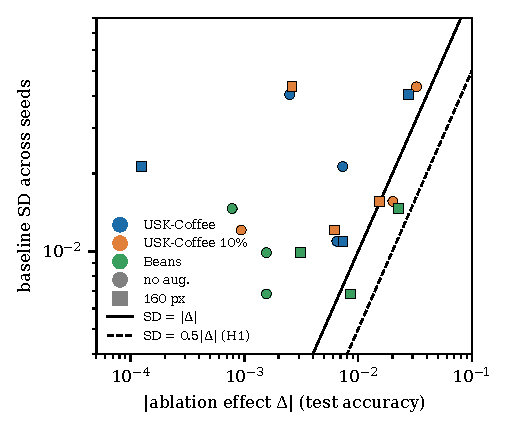
\includegraphics[width=0.6\linewidth]{fig_noise_effect.pdf}
\caption{Baseline SD across seeds against the absolute ablation effect, one
point per cell. Points above the dashed line satisfy H1; points above the solid
line have more seed noise than effect.}
\label{fig:noise}
\end{figure}

\paragraph{H2: one seed often points the wrong way (\HTwo{}).} With $k=1$, the
reversal rate ranged from \KOneMin{} to \KOneMax{} (median \KOneMedian{}), above
10\% in every dataset. More seeds helped unevenly (Figure~\ref{fig:reversal}):
with $k=5$ the rate was still above 10\% in \NKFiveAbove{} of \NCells{} cells.

\begin{figure*}[t]
\centering
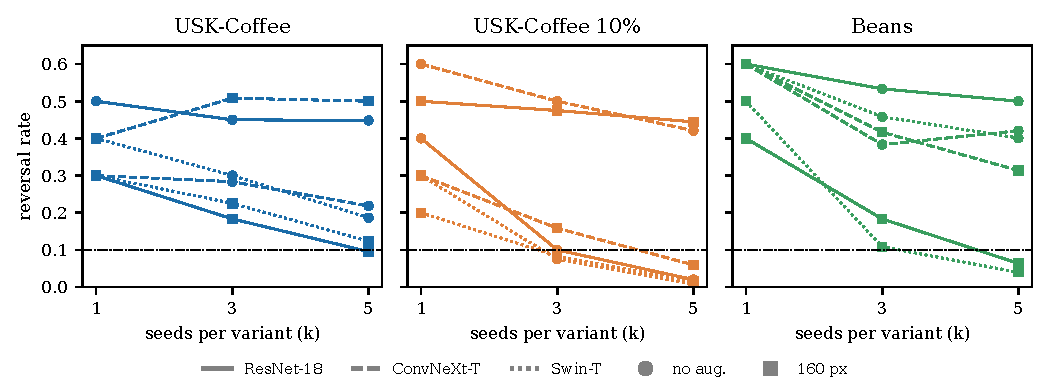
\includegraphics[width=\linewidth]{fig_reversal.pdf}
\caption{Reversal rate as a function of the seeds per variant, one line per
cell. The dash-dotted line marks 10\%.}
\label{fig:reversal}
\end{figure*}

\paragraph{How many seeds.} No ablation effect was significant after Holm
correction with ten seeds (\NHolm{} of \NCells{}). The bootstrap CI excluded
zero in \NCIExcludes{} cells whose paired test did not reach 0.05 even before
correction; we report the pre-registered test as primary and note that the two
procedures disagree at this sample size. The replicated comparison also tests
the two ablations against each other, which the protocol did not register: of
these \NExploratory{} exploratory contrasts, \NExploratoryHolm{} survived Holm
correction, \ExploratoryPair{} on \ExploratoryCell{}
($\Delta=\ExploratoryDelta{}$, $p=\ExploratoryP{}$). The seeds needed for 80\% power ranged
from \PowerMin{} to the hundreds of thousands, with median \PowerMedian{}; no
cell needed ten or fewer. Reaching a reversal rate of at most 10\% within five
seeds happened in \NStableCNN{} of \NCellsCNN{} CNN cells and \NStableTr{} of
\NCellsTr{} transformer cells; with one transformer this is a description, not a
test.

\paragraph{H3: less data did not mean more seed noise (\HThree{}).} On the 10\%
subset the seed SD rose for ResNet-18 (\SDFullRes{} to \SDTenRes{}) and Swin-T
(\SDFullSwin{} to \SDTenSwin{}) but fell for ConvNeXt-T (\SDFullConv{} to
\SDTenConv{}), so H3 is rejected as pre-registered.

\paragraph{Which seed versus which test images.} The half-width of the test-set
CI was below the seed SD in only \NEvalBelow{} of \NPairs{}
dataset--architecture pairs. The finite test set is a second source of
uncertainty of the same order as the seed, and a single-seed result carries
both.

\section{Discussion}\label{sec:discussion}

The ablations we chose are small on purpose: they are the changes an applied
paper reports in its ablation table. For changes of that size, on datasets of
this size, one run per variant does not support a claim in either direction,
and even ten paired seeds did not separate any effect from zero after
correction. Three practical consequences follow. First, report the seed SD next
to any ablation effect; when the ratio is above one, the ablation is not
informative at that number of seeds. Second, plan the number of seeds from a
pilot's paired differences rather than by habit; the power figures in
Table~\ref{tab:cells} show that most effects below one point of accuracy need
more seeds than a single-GPU project can run. Third, the test set's own uncertainty
belongs in the same report.

\paragraph{Limitations.} One GPU and one software stack; three datasets, all
agricultural and with few classes; ablations small by design, so the results
say nothing about large changes; accuracy as the primary metric (macro-F1 is
recorded in the release but carried no hypothesis); a single transformer, so
the CNN--transformer contrast is descriptive; one subset draw for the 10\%
regime.

\section*{Reproducibility}
The protocol, its deviation, the per-run reports and \texttt{run.json} records,
the analysis code and its tests, and the script that generates every number,
table and figure in this paper are in
\url{https://github.com/marcus-vreis/VisionForge} under
\texttt{research/seed\_variance/}. \todo{Archive the study folder on Zenodo and
cite that DOI here.}

\section*{Use of generative AI}
Generative AI coding assistants (Anthropic's Claude through Claude Code,
OpenAI's Codex and Google's Gemini) were used to draft code, tests and parts of
this text. The author designed the study, pre-registered it, ran it, checked
every number against the generated sources and every reference against its
source, and takes full responsibility for the paper.

\bibliographystyle{plainnat}
\bibliography{refs}

\end{document}
